\chapter{Introducción}\label{ch:introduccion}


\section{Motivación y contexto}\label{sec:motivacion-y-contexto}
A día de hoy, gracias a los avances en ciencias de la computación, la inteligencia artificial (en adelante IA) se está
convirtiendo en una parte fundamental de la atención médica actual.
Algoritmos y aplicaciones impulsadas por IA se usan en el día a día para ayudar a los profesionales en entornos clínicos
y en el ámbito de la investigación.

Según la Confederación Española de Alzheimer (CEAFA)~\cite{ceafa} la \textbf{Enfermedad del Alzheimer} (en adelante EA)
es una enfermedad neurodegenerativa que afecta a aproximadamente 1.200.000 personas en España y a más de 50 millones de
personas en el mundo según un artículo de la Universitat Oberta de Catalunya (UOC)~\cite{uoc}.
Es una enfermedad progresiva, o lo que es lo mismo, que empeora con el tiempo y para la que no existe una cura, solo
la posibilidad de aplicar tratamientos que ralenticen su avance.
Para que estos tratamientos no resulten perjudiciales para la salud del paciente deben realizarse en las primeras etapas
de la enfermedad.
Por ello un diagnóstico temprano puede ser determinante para el paciente, pero, en la mayoría de casos, detectar esta
enfermedad en las primeras fases de la misma es una tarea muy compleja.

Investigaciones previas han concluido que las primeras lesiones cerebrales pueden aparecer incluso 20 años antes de que
aparezcan los primeros síntomas del Alzheimer~\cite{ceafa}.
De hecho una de las evaluaciones médicas para la detección de la enfermedad se basa en el diagnóstico por imágenes
cerebrales mediante la realización de un examen imagenológico, que puede incluir técnicas como: Imagen por Resonancia
Magnética (en adelante MRI), Tomografía Computarizada o Tomografía por emisión de positrones (en adelante PET).

A día de hoy el aprendizaje profundo o deep learning (en adelante DL)  ha levantado mucho interés en el mundo de la
medicina.
El Deep learning es un subconjunto del machine learning (en adelante ML) en IA, que simula el comportamiento del cerebro
humano en el procesamiento de datos y el reconocimiento de patrones para resolver problemas complejos de toma de
decisiones.

Es por esto que el uso de DL puede ayudar a un diagnóstico temprano, ya que estos sistemas pueden ser utilizados para la
detección de anomalías en imágenes médicas donde destaca la rapidez de la detección, sirviendo como herramienta de
prevención y seguimiento de la enfermedad.

También cabe destacar que la enfermedad del Alzheimer presenta diferentes fases y la velocidad a la que avanza la
enfermedad por las diferentes fases varía, por lo que es más difícil realizar predicciones a largo plazo.
Se usan escalas con distinto número de fases:
\begin{itemize}
    \item \textbf{La escala de deterioro global (GDS)}~\cite{gds} se divide en siete fases que dependen del valor del
    deterioro cognitivo y más común utilizarla para escalar la demencia senil.
    Sus fases son: ausencia de alteración cognitiva, disminución cognitiva muy leve, defecto cognitivo leve, defecto
    cognitivo moderado, defecto cognitivo moderado-grave, defecto cognitivo grave y defecto cognitivo muy grave.
    \item \textbf{La escala de clasificación de la demencia clínica (CDR)}~\cite{cdr} se divide en cinco fases, es la más
    utilizada en el área de investigación y evalúa diferentes parámetros como la memoria, la orientación, la resolución
    de problemas, el juicio, etc.
    Sus fases son: Cognitivamente sano (CDR 0), demencia cuestionable (CDR 0.5), demencia leve (CDR 1), demencia
    moderada (CDR 2) y demencia grave (CDR 3).
    \item \textbf{La escala de clasificación común}~\cite{alz-org-etapas} solo tiene en cuenta tres fases, es la más
    usada en la comunicación médico-familia, ya que es la más sencilla de comprender.
    Las fases que tiene en cuenta son: Enfermedad de Alzheimer leve (etapa temprana), enfermedad de Alzheimer moderada
    (etapa media) y enfermedad de Alzheimer grave (etapa final).\\
\end{itemize}

A día de hoy, realizar estudios en esta área significa conseguir grandes avances en el mundo de la medicina y del
diagnóstico del Alzheimer, ayudando a mejorar la vida de los pacientes y las familias.
Por lo tanto, la motivación de este trabajo se centra en el estudio del uso de técnicas de Deep Learning para el
diagnóstico del Alzheimer a partir de imágenes cerebrales.

\section{Alzheimer}\label{sec:alzheimer}
El Alzheimer es una enfermedad neurodegenerativa, progresiva, irreversible y terminal en la que se produce una pérdida
de neuronas principalmente relacionada con dos tipos de alteraciones cerebrales: la acumulación anormal de placas
seniles de proteína beta-amiloide y ovillos neurofibrilares de proteína Tau~\cite{ceafa}.

\subsection{Epidemiología de la enfermedad}\label{subsec:epidemiologia}
Es la forma más común de demencia, una pérdida de la función cerebral que afecta la memoria, el pensamiento, el
lenguaje, el juicio y el comportamiento.
Se estima que entre un 60 y un 80 por ciento de los casos de demencia se producen a causa de la EA en los países
desarrollados~\cite{alz-org-enfermedad}.

Esta patología tiene una mayor frecuencia en personas mayores de 65 años, siendo la prevalencia de un 7\% en este grupo
de población, y aproximándose al 50\% en mayores de 85 años~\cite{ceafa}.
Aunque en otros casos más extremos y mucho menos frecuentes puede ser desarrollada a partir de los 30 años, siendo
denominada en este caso como Enfermedad de Alzheimer precoz o de aparición temprana~\cite{mayo-clinic-alz-precoz}.
En término medio, una persona con Alzheimer vive de 4 a 8 años después de ser diagnosticada, pero puede vivir hasta 20
años dependiendo de otros factores como es, por ejemplo, la etapa en la que se diagnostique la enfermedad~\cite{alz-org-etapas}.

Actualmente, en España la cifra de personas afectadas por la enfermedad del Alzheimer es de aproximadamente 1.200.000,
acercándose a las 5.000.000 personas si contamos con la familia~\cite{ceafa}.

\subsection{Cuadro clínico}\label{subsec:cuadro-clinico}
Las lesiones cerebrales características de la EA comienzan años antes de que aparezcan los primeros síntomas, según
concluyen algunas investigaciones, estas alteraciones cerebrales pueden darse entre 10 o 20 años antes.

La EA produce en el cerebro una pérdida neuronal progresiva que se relaciona de manera directa con la acumulación de
placas de proteína beta-amiloide y de ovillos neurofibrilares de proteína Tau que impiden a las neuronas comunicarse
entre sí conduciendo a su muerte.
El conjunto de estas lesiones se inicia en el hipocampo y se distribuye a otras regiones cerebrales según el grado de
evolución de la enfermedad.

El hipocampo es una de las áreas del cerebro cuyo funcionamiento es vital para la memoria y el aprendizaje.
Este es el motivo por el cual, en las primeras etapas de la enfermedad, las personas con EA presentan dificultades para
recordar sucesos recientes o para retener información nueva, sin embargo, se conservan recuerdos del pasado porque las
zonas del cerebro implicadas todavía no se han visto afectadas.

La afectación progresiva de otras áreas cerebrales da lugar a la aparición de otros síntomas que afectan a la toma de
decisiones, cambios conductuales y de personalidad, dificultad para la comunicación y la pérdida de funciones biológicas
que conlleva la muerte.

El desarrollo progresivo de la EA es lo que da lugar a que se establezca una distinción de etapas de la enfermedad según
la evolución de las lesiones en el cerebro y según la evolución de los síntomas que van produciendo esos daños.
Distinguiendo tres etapas: \textbf{Enfermedad de Alzheimer leve} (etapa temprana), \textbf{Enfermedad de Alzheimer moderada}
(etapa media) y \textbf{Enfermedad de Alzheimer grave} (etapa final), las cuales se detallan posteriormente~\cite{alz-org-etapas}.

\subsection{Cómo afecta al funcionamiento cerebral la acumulación de proteína beta-amiloide y Tau}
\label{subsec:acumulacion-proteínas}
La acumulación en el cerebro de placas de proteína \textit{beta-amiloide} y de ovillos neurofibrilares de proteína
\textit{Tau} provoca la interrupción de la comunicación, el metabolismo y la reparación de neuronas, que son los
procesos que hacen que las neuronas se mantengan sanas.
La suspensión de estos procesos provoca la muerte de neuronas, y es la que conlleva problemas de memoria.

La proteína \textit{beta-amiloide} es una proteína presente en el cerebro que lleva a cabo determinadas funciones fisiológicas.
En una persona con EA, la eliminación de los restos de esta proteína no se realiza de manera correcta, provocando la
formación de placas seniles (depósitos extracelulares de \textit{beta-amiloide}) y afectando al funcionamiento cerebral normal.

La proteína \textit{Tau} tiene como principal objetivo mantener la estructura de las neuronas.
En personas con EA, se provoca una serie de alteraciones bioquímicas que causan la formación de ovillos neurofibrilares
como un conglomerado anormal de proteínas que se compone de pequeñas fibrillas entrelazadas en el interior de las
neuronas~\cite{fund-pasqual-maragall-afectacion-cerebral}.

A medida que las neuronas mueren y las conexiones entre las redes de neuronas se rompen, muchas regiones del cerebro
comienzan a encogerse.
En la etapa final de la EA, el daño cerebral producido es muy grande, resultando una pérdida significativa del volumen
de tejido cerebral~\cite{img-cambios-cerebrales}.

\begin{figure}[H]
    \centering
    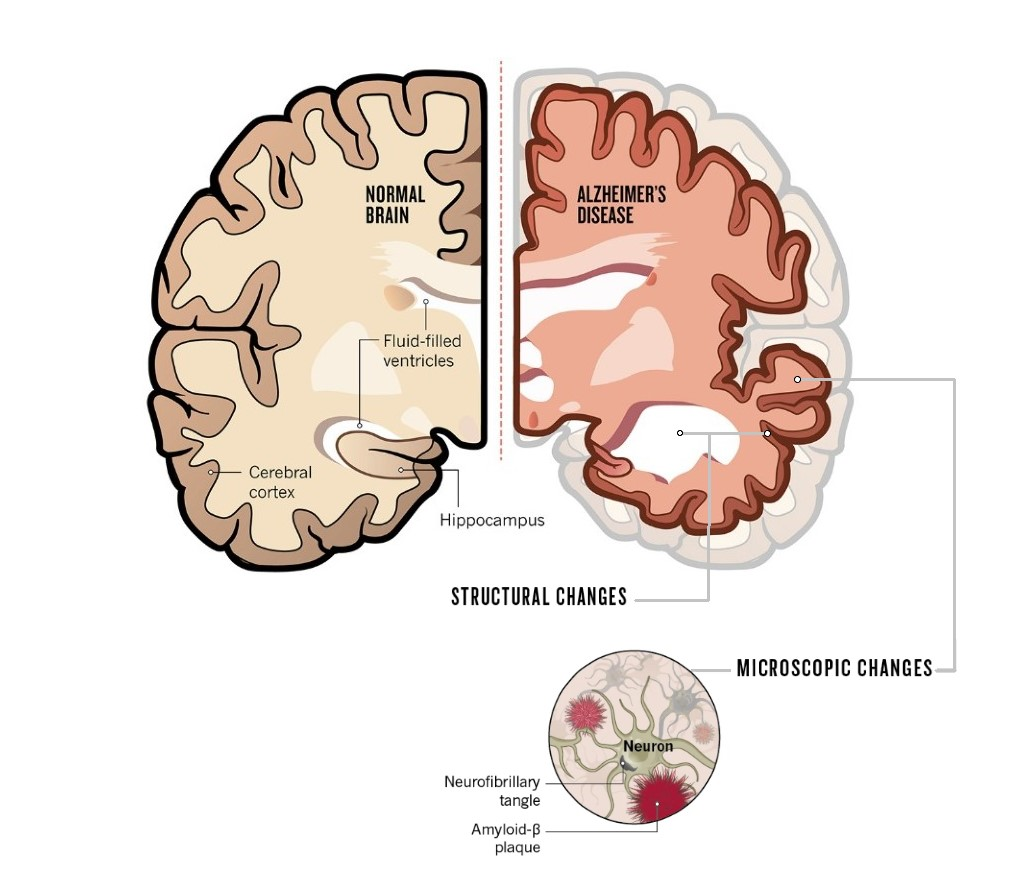
\includegraphics[width=\textwidth]{./imgs/lesiones-cerebrales}
    \caption{Lesiones cerebrales producidas por la enfermedad de Alzheimer.\\Imagen adaptada de una
    ilustración de Stacy Jannis, Alzheimer\'s Association~\cite{nature}.}
    \label{fig:lesiones-cerebrales}
\end{figure}

\subsection{Fases de la enfermedad}\label{subsec:fases-enfermedad}
La EA es una enfermedad de larga evolución en la que, usando una escala de clasificación común, se distinguen
tres fases~\cite{alz-org-etapas}.

\subsubsection{Enfermedad de Alzheimer leve}\label{subsubsec:etapa-temprana-EA}
Esta etapa se conoce como etapa temprana y permite al paciente desenvolverse de forma independiente, pero aparecen los
fallos de memoria, como son:
\begin{itemize}
    \item Dificultad para encontrar la palabra o el nombre correctos.
    \item Problemas para realizar tareas en entornos sociales o laborales, destacando la presencia de cambios de
    personalidad.
    \item Olvidarse de algo que acaba de leer.
    \item Problemas para encontrar objetos.
    \item Dificultad para recordar acontecimientos y conversaciones recientes.\\
\end{itemize}

Realizar un diagnóstico de la enfermedad en esta etapa puede ser determinante, ya que existe la posibilidad de aplicar
tratamientos con los que la evolución de la enfermedad pueda ralentizarse sin que resulten perjudiciales para la salud
del paciente.
Sin embargo, es muy difícil realizar el diagnóstico en esta fase pues la mayoría de los síntomas se suelen confundir con
conductas características de la vejez.

\subsubsection{Enfermedad de Alzheimer moderada}\label{subsubsec:etapa-media-EA}
En esta etapa media comienzan las limitaciones en las actividades de la vida diaria y la persona con EA necesita un
nivel de atención mayor en tareas básicas como la alimentación o el aseo personal.

La memoria se sigue viendo afectada, de manera más pronunciada en esta etapa, como puede ser dificultad para reconocer a
miembros de la familia, olvidarse eventos o información de la historia personal, o el aumento del riesgo de
desorientarse y perderse en lugares conocidos.

\subsubsection{Enfermedad de Alzheimer grave}\label{subsubsec:etapa-final-EA}
En esta etapa final las personas con EA pierden la capacidad de responder a su entorno, sufriendo una pérdida completa
de la memoria y las capacidades intelectuales y funcionales.
Provocando la necesidad de cuidado y asistencia absoluta.
Se produce una pérdida progresiva del lenguaje haciendo que el paciente deje de hablar y una posterior inmovilidad
completa.

La pérdida de las capacidades funcionales hace que se produzca una pérdida de peso y disminución de sus defensas
inmunológicas que conllevan a la muerte.

\subsection{Diagnóstico de la enfermedad}\label{subsec:diagnostico-enfermedad}
Para diagnosticar la EA se requiere de evaluaciones médicas exhaustivas, en las que se evalúa el deterioro de la memoria,
la presencia de cambios de conducta y el estado de otras habilidades de razonamiento, que permitan determinar cuáles son
las capacidades funcionales.
Además, es necesario realizar pruebas médicas que descarten otras posibles causas de deterioro.

El diagnóstico se puede dividir en cuatro partes~\cite{mayo-clinic-diagnostico,alz-org-diagnostico}~:
\begin{itemize}
    \item \textbf{Evaluación del estado mental}: Se evalúan las habilidades de razonamiento (cognitivas) y memoria.
    \item \textbf{Examen físico}: Se evalúa la salud general de la persona, para descartar otras afecciones tratables
    que causen síntomas similares.
    \item \textbf{Examen neurológico}: Se realiza una evaluación de afecciones cerebrales y de salud mental, descartando
    algún trastorno como la depresión.
    \item \textbf{Pruebas de laboratorio} y \textbf{estudios de imágenes cerebrales}.\\
\end{itemize}

\subsubsection{Pruebas de laboratorio}\label{subsubsec:pruebas-laboratorio-EA}
Las pruebas de laboratorio incluyen: análisis de sangre para descartar otros trastornos, o examen del líquido
cefalorraquídeo para medir los niveles de proteína amiloide y tau, determinando según su proporción si se trata de EA.
Los exámenes del líquido cefalorraquídeo solo se realizan en casos atípicos y de rápida evolución.

\subsubsection{Pruebas de diagnóstico por imágenes}\label{subsubsec:pruebas-imagenes-EA}
Las pruebas de diagnóstico por imágenes ayudan a distinguir diferentes tipos de enfermedades cerebrales degenerativas y
además establecer cuál es el grado de degeneración, por lo que son las pruebas más fiables para el diagnóstico del
Alzheimer.

Las técnicas más frecuentes de diagnóstico por imágenes son:
\begin{itemize}
    \item \textbf{Imagen por Resonancia Magnética (MRI)}: Es una técnica no invasiva que a través de campos magnéticos
    genera imágenes anatómicas tridimensionales.
    Proporciona información exhaustiva de los tejidos blandos y permite examinar la anatomía del cerebro y evaluar
    lesiones presentes.
    \item \textbf{Tomografía Computarizada (más conocida como TAC)}: Con esta técnica se recopilan imágenes transversales
    sucesivas mediante rayos X. Proporciona imágenes óseas, de tejidos blandos y aire y permite identificar anomalías
    asociadas al Alzheimer.
    \item \textbf{Tomografía por emisión de positrones (PET)}: Esta técnica usa radiofármacos de administración intravenosa
    gracias a los cuales se obtienen imágenes de alta definición en las que se pueden detectar y visualizar depósitos
    extracelulares de proteína beta-amiloide.\\
\end{itemize}

\begin{figure}[H]
    \centering
    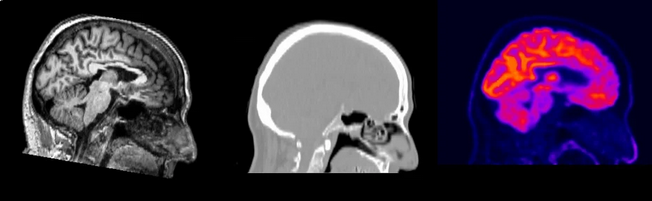
\includegraphics[width=\textwidth]{./imgs/MRI-TAC-PET}
    \caption{Técnicas de diagnóstico por imágenes de la enfermedad de Alzheimer.\\ De izquierda a derecha: MRI, TAC y PET.
    \\Fuente: Fundación Pasqual Maragall~\cite{img-mri-tac-pet}.}
    \label{fig:tecnicas-diagnosico-imagen}
\end{figure}

\section{Estado del arte}\label{sec:estado-del-arte}
En este apartado se incluye la situación actual del uso de técnicas de DL para el diagnóstico del Alzheimer, es decir,
la información sobre las últimas actualizaciones e investigaciones ya disponibles al público sobre este tema.

En la última década, las técnicas de aprendizaje profundo han alcanzado una enorme popularidad en el ámbito del análisis
de imágenes médicas y como herramienta de diagnóstico y seguimiento de enfermedades.
Al mismo tiempo, ha incrementado el uso de técnicas de neuroimagen para el diagnóstico de la EA, por lo que la unión de
ambas técnicas, de aprendizaje profundo y de neuroimagen, ha demostrado ser una combinación ideal para realizar un
correcto diagnóstico de la enfermedad y poder predecir la evolución de la misma.

El número de artículos de investigación de la detección de la EA que se han publicado en los últimos años ha crecido
exponencialmente.
Recogiendo información sobre múltiples resultados con el uso de distintos biomarcadores o distintos modelos profundos.

La mayoría de los artículos publicados tratan el tema de la misma manera: planteando un nuevo modelo de aprendizaje
profundo y no llegando a explorar mejoras a otras alternativas o reflexionar sobre qué recursos son mejores, siendo el
resultado un cúmulo de estudios que no producen una conclusión concreta a qué métodos son más óptimos y por qué.
Existe un artículo de la universidad en Newcastle, Australia, que realiza una revisión de la literatura de más de 100
artículos y que detalla los hallazgos y tendencias, examinando biomarcadores y características útiles, técnicas de
preprocesamiento necesarias y diferentes métodos de tratamiento de neuroimágenes~\cite{literature-review}.
Este estudio se ha utilizado de referencia para este apartado.

\subsection{Biomarcadores que intervienen en la detección de la EA}\label{subsec:biomarcadores-estado-del-arte}
Para la detección de la EA las técnicas de neuroimagen no invasivas más utilizadas en los estudios son: MRI, fMRI
(Imagen por resonancia magnética funcional)  y PET.

La fMRI es un tipo especial de MRI que proporciona un conjunto de imágenes del flujo sanguíneo de ciertas partes del
cerebro y también son utilizadas para evaluar daños cerebrales~\cite{mayo-clinic-mri}.

De estas técnicas, MRI es el biomarcador más utilizado en la literatura debido a que ha demostrado un alto rendimiento.
A pesar de que varios estudios han demostrado que la MRI es más discriminatoria en comparación con la PET, otros estiman
que la MRI es igual de discriminatoria que la PET o ligeramente menos.

Además MRI es la técnica más frecuente en las pruebas médicas para la detección de la EA ya que proporciona información
precisa y el coste de su realización es menor.
Lo que sitúa a esta técnica como la mejor candidata para avanzar en la investigación del diagnóstico de la enfermedad.

\subsection{Técnicas de preprocesamiento de biomarcadores}\label{subsec:preprocesamiento-estado-del-arte}
La mayoría de los trabajos de investigación, en especial los de ML, necesitan aplicar un preprocesamiento a los datos
antes de poder manejarlos.
Con el uso de técnicas de DL, algunos pasos de preprocesamiento no son tan cruciales, no obstante, en la mayoría de
casos, se realiza un preprocesamiento de los datos.
Las técnicas de preprocesamiento más usadas son:
\begin{itemize}
    \item Normalización de la intensidad.
    \item Registro de la imagen.
    \item Segmentación del tejido.
    \item Segmentación del cráneo.
    \item Corrección del movimiento.\\
\end{itemize}

\subsection{Técnicas de análisis de neuroimagen}\label{subsec:analisis-de neuroimagen-estado-del-arte}
Las técnicas de análisis o de extracción de características en neuroimagen se pueden dividir en cuatro categorías,
dependiendo de las características extraídas: basadas en vóxeles, en cortes, en parches y en regiones de interés
(en adelante ROI).

\textbf{La técnica basada en vóxeles}, también llamada morfometría basada en Vóxel (VBM), es la más sencilla, se utiliza en MRI,
permite el análisis de lesiones focales cerebrales y en ella se realiza una división del cerebro en vóxeles que son la
unidad cúbica que compone un objeto tridimensional, el equivalente al píxel en un objeto bidimensional.
Esta técnica permite identificar las diferencias de concentración entre la sustancia gris y la sustancia blanca del
cerebro mediante la comparación vóxel a vóxel de los valores de intensidad de los mismos.

\textbf{La técnica basada en cortes} consiste en extraer, mediante cortes, imágenes bidimensionales con la mayor información
posible.
Ya que el uso de las tres vistas de las neuroimágenes tridimensionales puede proporcionar características
útiles adicionales para la clasificación, algunos estudios tienen en cuenta todas las vistas de la imagen (sagital,
coronal y axial).

En \textbf{la técnica basada en parches}, pequeños sub-volúmenes de la imagen definidos como cubos tridimensionales conocidos
como parches se usan para extraer patrones relacionados con la enfermedad.
La diferencia entre un parche y un vóxel es que los vóxeles constituyen la mínima unidad procesable.

La \textbf{técnica basada en ROI} se centra en las partes del cerebro más afectadas en la fase temprana de la EA, en vez de
ocuparse de todo el cerebro.

Las conclusiones obtenidas en la literatura sobre las técnicas de análisis en neuroimagen son las siguientes:
\begin{itemize}
    \item Los métodos basados en ROI y en parches son más exactos, ya que son los métodos con los que se obtiene
    información más relevante;
    sin embargo, son también los métodos más costosos.
    \item Los métodos basados en parches son más precisos que los basados en vóxeles, pero la selección de los parches
    con más información de la imagen es una tarea compleja.
    \item El uso de cortes 2D como entrada en lugar de la imagen 3D en su totalidad evita la generación de millones de
    parámetros de entrenamiento e induce a la simplificación de las redes a costa de perder información.
    \item Al utilizar métodos basados en cortes, las vistas sagital y coronal resultan ser las más discriminatorias,
    aunque las vistas axiales son las más utilizadas.
    Hay estudios que afirman que no hay diferencias significativas entre planos.\\
\end{itemize}

\subsection{Modelos profundos más utilizados para obtener patrones relacionados con la EA}
\label{subsec:modelos-profundos-estado-del-arte}
Lamentablemente la mayoría de los estudios no publican su código fuente por lo que resulta difícil comparar de manera
imparcial los estudios entre sí.
Además, normalmente los artículos se limitan a comparar precisiones finales y no a comparar distintos factores como el
coste computacional.

Las redes neuronales convolucionales (en adelante CNN) son las más usadas en el ámbito de la medicina porque han
demostrado una alta precisión en términos de clasificación de imágenes médicas.

Entre los modelos observados, los mejores resultados se encuentran entre las 3D-CNN y las 2D-CNN. Ambas opciones tienen
un buen rendimiento para la extracción de características, en el caso de las arquitecturas de red neuronal de tipo
3D-CNN estas muestran ligeramente un mayor rendimiento, ya que recogen información tridimensional y, por tanto, más
cantidad de información;
sin embargo, las de tipo 2D-CNN son más fáciles de entrenar, requieren de un menor coste computacional.

En cuanto a arquitecturas 2D-CNN: Inception-V4, ResNet y CaffeNet han superado a GoogLeNet, VGGNet-16 y AlexNet.

En la mayor parte de los estudios se entrena un modelo profundo desde cero, pero, esto puede ser ineficiente, porque
el proceso de entrenamiento requiere mucho tiempo y un gran conjunto de datos.
Mientras que los conjuntos de datos para la detección y clasificación de objetos genéricos cuentan con millones de
imágenes, los conjuntos de datos de neuroimagen disponibles del seguimiento de la EA suelen ser pequeños, de solo
cientos de imágenes, lo que da lugar a un sobreajuste.
El Transfer Learning (en adelante TL) es más rápido y alcanza mejores resultados que el entrenamiento desde cero, de
modo que, generalmente resulta útil utilizar CNNs probadas y pre-entrenadas para volver a entrenarlas con otro conjunto
de datos.

\subsection{Conjuntos de datos y herramientas de software útiles}\label{subsec:datos-y-herramientas-estado-del-arte}
Como paquetes software de análisis de neuroimagen están:
FreeSurfer\footnote{\href{https://surfer.nmr.mgh.harvard.edu/}{FreeSurfer}},
FSL\footnote{Functional magnetic resonance imaging of the brain Software Library, \href{https://fsl.fmrib.ox.ac.uk/fsl/fslwiki/}{FSL}},
MIPAV\footnote{Medical Image Processing, Analysis, and Visualization, \href{https://mipav.cit.nih.gov/}{MIPAV}}
y SPM\footnote{Statistical Parameter Mapping, \href{https://www.fil.ion.ucl.ac.uk/spm/}{SPM}},
que ofrecen herramientas potentes para diversas técnicas de preprocesamiento automatizado comentadas en el
apartado~\ref{subsec:preprocesamiento-estado-del-arte}.

Para implementar modelos profundos las herramientas más utilizadas son:
MATLAB\footnote{\href{https://www.mathworks.com/products/matlab.html}{MATLAB}}
Keras\footnote{\href{https://keras.io/}{Keras}},
TensorFlow\footnote{\href{https://www.tensorflow.org/}{TensorFlow}},
Theano,
Caffe\footnote{\href{https://caffe.berkeleyvision.org/}{Caffe}},
y Torch\footnote{\href{http://torch.ch/}{Torch}}.
Siendo Keras y TensorFlow los más utilizados y Torch el menos utilizado.

La principal dificultad a la que se enfrentan los investigadores es la falta de imágenes que permitan formar un gran
conjunto de datos de entrenamiento con el que poder obtener un resultado preciso y, por tanto, un diagnóstico fiable.
La escasez de datos es un problema que se debe a las restricciones de privacidad de las imágenes médicas y de su elevado
coste en muchos casos.

Como bases de datos online para obtener conjuntos de datos relativos a la EA, las más importantes son:
ADNI\footnote{Alzheimer’s Disease Neuroimaging Initiative, \href{https://adni.loni.usc.edu/}{ADNI}},
AIBL\footnote{Australian Imaging, Biomarker and Lifestyle, \href{https://aibl.csiro.au/}{AIBL}},
OASIS\footnote{Open Access Series of Imaging Studies, \href{https://www.oasis-brains.org/}{OASIS}}
y MIRIAD\footnote{Minimal Interval Resonance Imaging in Alzheimer's Disease,
    \href{https://www.ucl.ac.uk/drc/research/research-methods/minimal-interval-resonance-imaging-alzheimers-disease-miriad}{MIRIAD}},
que ofrecen al público biomarcadores como neuroimagen, información genética y sanguínea, y evaluaciones
clínicas y cognitivas.
ADNI es la que más destaca de todas ellas por ser un estudio multicéntrico y longitudinal, además es el más común en la
literatura, de manera individual o en combinación con otros.
Esta última es una forma de poner solución a la insuficiencia de datos.
Al combinar diferentes conjuntos de datos, se produce una mayor heterogeneidad, lo cual es una desventaja, pero se crea
un modelo amplio para la clasificación y la predicción.

Las técnicas de aumento de datos entre las que se encuentran la reflexión, la rotación, la traslación aleatoria, el
desenfoque o el escalado mejoran el rendimiento de la clasificación sin la necesidad de recoger nuevos datos cuando
estos son limitados.

Se recomienda el uso de un conjunto de datos equilibrado, ya que, en caso contrario, un desequilibrio entre pacientes de
distintas categorías provoca una variación en la precisión.
Siendo, por tanto, preferible el uso de un conjunto de datos menor antes que uno desequilibrado.

%\section{Objetivos}
%\input{secciones/01-4_Objetivos}
%
%\section{Alcance y metodología}
%\input{secciones/01-5_AlcanceMetodologia}